\documentclass[
    aps,
    prl,
    reprint,
    10pt,
    amsmath,
    amssymb,
    a4paper,
    longbibliography
]{revtex4-2}

\usepackage{
    graphicx,
    dcolumn,
    amsmath,
    amsfonts,
    amsthm,
    datetime,
    hyperref,
}
\usepackage[separate-uncertainty=true]{siunitx}
\usepackage[usestackEOL]{stackengine}
\usepackage[margin=2cm]{geometry}
\graphicspath{{figures/}}
\bibliographystyle{apsrev}

\begin{document}

\title{Time of flight refractometry of air, acrylic and water}
\author{T.D. Schanzer (z5310829)}
\affiliation{
    School of Physics, %
    University of New South Wales, %
    Sydney NSW 2052, Australia
}
\collaboration{Cohort A, Monday 9 a.m.~---~12 p.m.}
\noaffiliation
\collaboration{2201 words}
\noaffiliation
\date{\currenttime~\today}

\begin{abstract}
    This report presents time-of-flight measurements of the speed of
    light and refractive
    index in air, poly(methyl methacrylate) (PMMA, commonly known as
    acrylic) and water using a simple teaching apparatus.
    The discrepancy between the results and values reported in literature
    is attributed to unavoidable misalignment of the apparatus, imperfect
    fabrication of
    the PMMA sample and water container, and drift in time measurements.
    An alternative method using refraction at the PMMA and water
    interfaces is proposed to eliminate these systematic errors.
\end{abstract}

\maketitle

\section{Introduction}

Measurements of the speed of light have a long history, with discussion of
whether or not it was finite traced back to the ancient Greeks.
R{\o}mer (1676) is usually credited with making the first accurate
measurements for his observation of variations in Io's eclipse durations
behind Jupiter as the Earth approached and receded in its annual orbit
\cite{spence_history}.

More sophisticated experiments later increased the precision with which
the speed of light was known, to the point that it could be given an
exact value in SI units in a 1983
resolution of the seventeenth General Conference on Weights and Measures.
Presently, the metre ``is defined by taking
the fixed numerical value of the speed of light in vacuum, $c$, to be
299 792 458 when expressed in the unit \si{\meter \per\second}''
\cite{sibrochure}.

The refractive index of a material is the factor by which it reduces the
speed and wavelength of light relative to the speed and wavelength in
vacuum. Refractometry, the measurement of refractive indices, has many
applications in modern research, industry and medicine. These include
concentration measurements of dissolved material in liquids (e.g., sugar
in drinks), characterisation of glasses and plastics (e.g., for use in
lenses) and analysis of biofluids (e.g., blood and urine)
\cite{meeten_measurement}.

\subsection{Modern Methods}
Modern refractometry methods are numerous. Meeten
\cite{meeten_measurement} describes several, including:

\emph{Interferometry.} An interferometer separates a laser into two beams,
one of which travels through air and the other through the medium of
interest, before recombining them to produce a pattern of interference
fringes from which the phase difference and refractive index can be
determined.

\emph{Deviation.} A beam of light is passed at an angle through a flat
sheet of the material with known thickness. The beam that emerges on the
other side of the sheet is parallel to the incident beam but offset
laterally due to refraction. The magnitude of the deviation can be
related to the refractive index, thickness and angle of incidence using
Snell's Law.

\emph{Critical angle (Abbe method).} The incidence angle at which light,
passing from the medium of interest into a medium of known lower
refractive index, is refracted at $\ang{90}$ is found by measuring the
reflectance or transmittance at the interface as a function of
incidence angle. The refractive index is easily calculated using Snell's
Law. This method is commonly used in commercial refractometers.

\subsection{The Refractive Index of Air}
Many experiments, including the one detailed here, are not conducted in
vacuum and must therefore account for the refractive index of air, which
is known to depend on wavelength, temperature, pressure and relative
humidity. A commonly-used empirical formula was developed by Edl{\'e}n
in 1966 and later revised by Birch and Downs in 1994 to better match
experimental results \cite{birchdowns}. The revised formula calculates
the refractive index in three steps: the first defines an intermediate
quantity
\begin{multline}
    n_\mathrm{s} = 1 + 10^{-8} \\
    \times \left(
        8342.54
        + 2406147 \left[
            130 - \left(\sigma / \si{\per\micro\meter}\right)^2
        \right]^{-1} \right. \\
        \left. + 15998 \left [
            38.9 - \left(\sigma / \si{\per\micro\meter}\right)^2
        \right]^{-1}
    \right)
    \label{edlen1}
\end{multline}
to account for dispersion (wavelength dependence);
$\sigma = 1/\lambda$ is the
wavenumber of the light in vacuum. The second step defines another
intermediate quantity
\begin{multline}
    n_\mathrm{tp} = 1 + \frac{(p / \si{\pascal})n_\mathrm{s}}{96095.43} \\
    \times \frac{
        \left[
            1 + 10^{-8} (0.601 - 0.00972 T / \si{\celsius})p / \si{\pascal}
        \right]
    }{
        1 + 0.003661 T / \si{\celsius}
    }
    \label{edlen2}
\end{multline}
accounting for the air pressure $p$ and temperature $T$. The final value
is
\begin{multline}
    n_\mathrm{a} = n_\mathrm{tp} - (f/\si{\pascal}) \\
    \times \left [
            3.7345 - 0.0401 \left(\sigma / \si{\per\micro\meter}\right)^2
    \right] \times 10^{-10},
    \label{edlen3}
\end{multline}
where $f$ is the partial pressure of water vapour.

The conditions measured in this experiment (using an inexpensive electronic
weather station) were
$T = \SI{20.4 \pm 1}{\celsius}$,
$p = \SI{1028 \pm 2}{\hecto\pascal}$ and
relative humidity $\mathrm{RH} = \SI{47 \pm 10}{\percent}$
with an estimated wavelength $\lambda = \SI{630}{\nano\meter}$. When
substituted into (\ref{edlen1}), (\ref{edlen2}) and (\ref{edlen3}),
these yield
\begin{equation}
    n_\mathrm{a} = 1.000275.
    \label{n_air_edlen}
\end{equation}
By comparison to experimental results, Birch and Downs
estimated the $1\sigma$ uncertainty of the formula to be $\SI{e-8}
{}$ \cite{birchdowns}, but given the uncertainty in $T$, $p$, $\mathrm
{RH}$ and $\lambda$ this is more likely to be on the order of $\SI
{e-6}{}$ \cite{emtoolbox}, which is nonetheless negligible in
comparison to the uncertainties in the results presented in this
report.


\section{Aim}

This experiment seeks to determine the speed of light and refractive
index in air, poly(methyl methacrylate) (PMMA, or acrylic) and water.


\section{Methods}

The experiment used a combined laser source and detector unit
(PHYWE 11226-99), containing a red laser source whose intensity was
modulated at $\SI{50}{\mega\hertz}$. The laser passed along an optical
bench to a reflector mounted at a variable position $x$, was reflected
back to the unit and directed onto a photodiode by a retro-reflector
\cite{datasheet}, as shown in Figure \ref{setup}.
The modulation of the laser intensity created pulses in
both the source signal and the intensity measured by the photodiode,
allowing the time difference between them to be measured on a digital
oscilloscope (Tektronix TBS-1072B) connected to the source/detector
unit. An illustration of this time measurement is shown in the top
panel of Figure \ref{setup}.

\begin{figure}[ht]
    \centering
    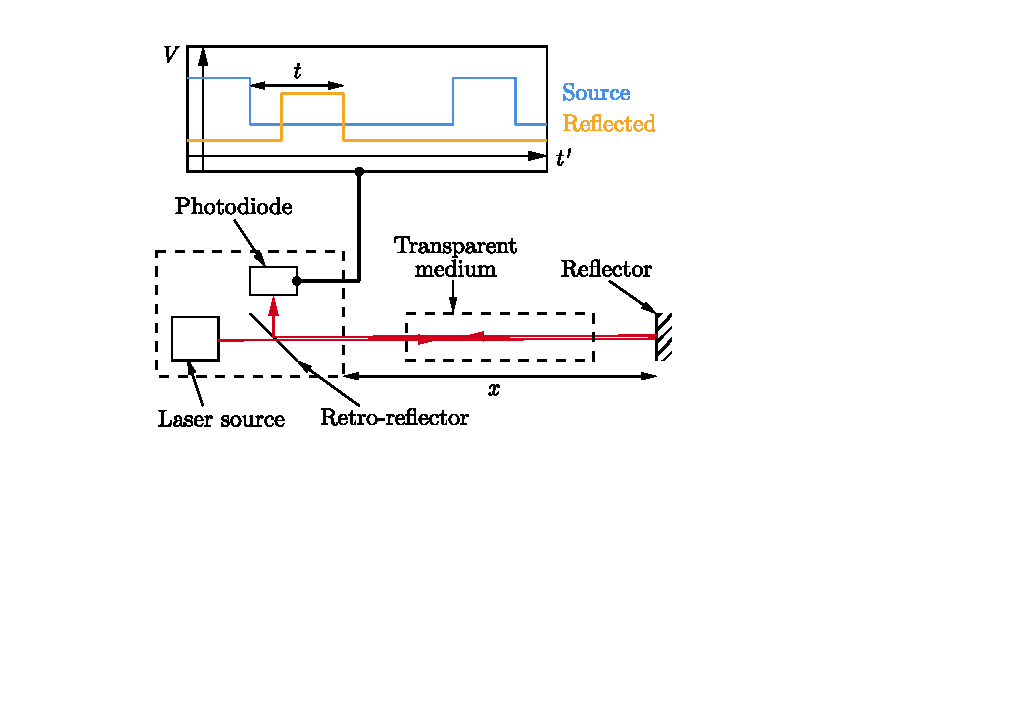
\includegraphics[width=\linewidth]{setup_updated}
    \caption{Experimental setup, showing model oscilloscope trace (top).}
    \label{setup}
\end{figure}

The speed of light in air, $c_\mathrm{a}$, was calculated by measuring
the time difference $t$ between the emitted and reflected beams as a
function of the reflector's position $x$ relative to a reference
point and performing a linear regression using the simple relation
\begin{equation}
    2x = c_\mathrm{a} t.
    \label{air_eqn}
\end{equation}

Two different approaches were compared for measuring the speed of
light in PMMA and water.

\emph{$\Delta x$ method.} A cylinder of the transparent medium was placed
in the path of the laser as shown in Figure \ref{setup} and the
source/detector unit calibrated to show a zero time difference between
the emitted and reflected beams. The cylinder was then removed,
shortening the time taken by the light, and the reflector moved horizontally
until the oscilloscope again showed a zero time difference, indicating
that the initial and final optical path lengths were equal. Mathematically,
\[
    2 n_\mathrm{a} x' = 2 n_\mathrm{a} (x - l) + 2 n_\mathrm{m} l,
\]
where $x$ and $x'$ are the initial and final reflector positions, $l$ is
the length of the cylinder and $n_\mathrm{m}$ is the refractive index of the
medium. Consequently, each measurement $(x,x')$ gives a value
\begin{equation}
    n_\mathrm{m} = \frac{n_\mathrm{a} (x' - x + l)}{l}.
    \label{x_eqn}
\end{equation}
An alternative is to calculate $n_\mathrm{m}$ from the $y$-intercept of
the linear regression of $x'$ on $x$, since it follows from
(\ref{x_eqn}) that
\begin{equation}
    x' = x + l \left( \frac{n_\mathrm{m}}{n_\mathrm{a}} - 1 \right).
    \label{x_int_eqn}
\end{equation}

\emph{$\Delta t$ method.} As before, the medium was placed in the optical
path and the source/detector unit calibrated to show a zero time
difference. The medium was removed and the resulting reduction in
travel time $\Delta t$ measured. Knowing that
\[
    \Delta t = 2 l \left(
        \frac{1}{c_\mathrm{m}} - \frac{1}{c_\mathrm{a}}
    \right),
\]
where $c_\mathrm{m}$ and $c_\mathrm{a}$ are the speeds of light in the
medium and air respectively, it follows that
\begin{equation}
    n_\mathrm{m} = \frac{c}{c_\mathrm{m}}
    = \frac{c \Delta t}{2 l} + \frac{c}{c_\mathrm{a}}.
    \label{t_eqn}
\end{equation}

The PMMA sample was a cylinder of length $\SI{0.491 \pm 0.001}{\meter}$.
The water was held in a plastic tube of length
$\SI{0.513 \pm 0.002}{\meter}$ that was capped at both ends with clear
plastic windows. Both lengths were measured using a tape measure.


\section{Results}

\subsection{Air}
The speed of light and refractive index in air were determined according
to (\ref{air_eqn}) by performing an ordinary least-squares linear
regression of $t$ on $2x$ and taking the reciprocal of the result.
This was necessary because ordinary least-squares regression only
accounts for errors in the response variable; $t$ was chosen as the
response because its uncertainty ($\SI{80}{\pico\second}$,
typically $2\%$, from the manual cursor positioning on the oscilloscope)
was more significant than that in $2x$ ($\SI{5}{\milli\meter}$,
typically $0.3\%$, due to possible misalignment). The results were
\begin{align*}
    c_\mathrm{a} &= \SI{2.941 \pm 0.016e8}{\meter \per\second}, \\
    n_\mathrm{a} &= \SI{1.019 \pm 0.005}{}.
\end{align*}
The uncertainty in $c_\mathrm{a}$ was obtained from the least-squares
regression algorithm (\verb|scipy.optimize.curve_fit| in Python),
and this was propagated to $n_\mathrm{a}$ using the standard
first-order Taylor expansion method. Despite realistic uncertainty
estimates, these values are not consistent with the accepted value
(\ref{n_air_edlen}), deviating by $3.6 \sigma$ or $1.9\%$.

Figure \ref{air_plot} shows the plot of $2x$ against $t$. The data points
fall consistently below the dashed expected line with the magnitude
of the deviation increasing with distance and time; given that the
orange regression line fits the points to within their uncertainties,
it is evident that a systematic error, rather than improper uncertainty
estimates, are responsible for the discrepancy in speed and refractive
index. Possible explanations are proposed in the Discussion.

\begin{figure}[ht]
    \centering
    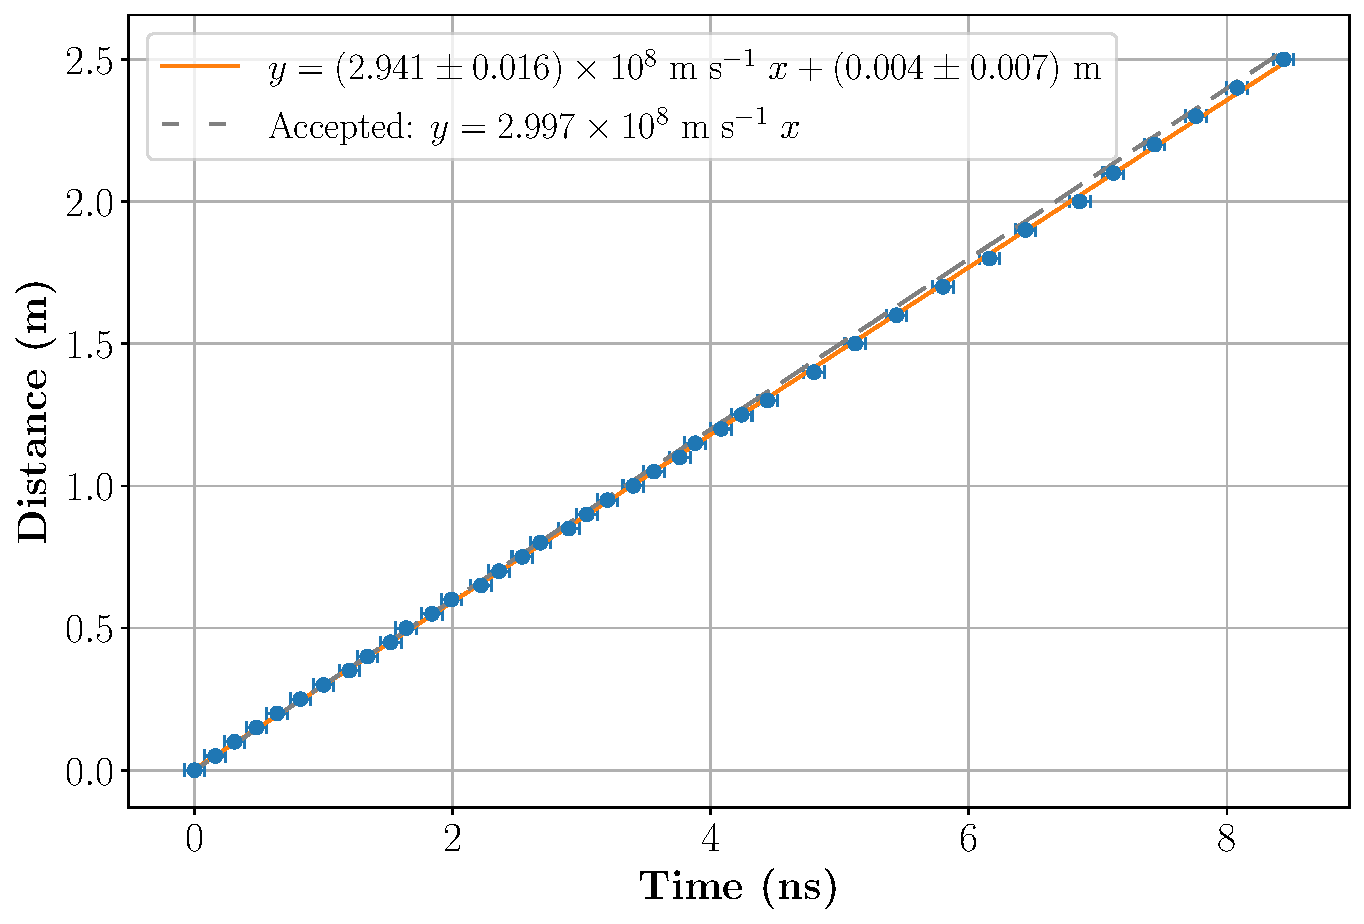
\includegraphics[width=\linewidth]{air}
    \caption{Plot of $2x$ vs. $t$ in air, with gradient $c_\mathrm{a}$.}
    \label{air_plot}
\end{figure}

\subsection{PMMA}
The speed of light and refractive index in PMMA were first calculated
two ways using the $\Delta x$ measurements described previously: using
(\ref{x_eqn}) for each pair of measurements $(x,x')$ and from the
intercept of the linear regression of $x'$ on $x$ according to
(\ref{x_int_eqn}). The values were also calculated for each $\Delta t$
measurement using (\ref{t_eqn}). The results are shown in Figure
\ref{acrylic_plot}; $\Delta x$ measurements were performed on two different
days but the result of intercept method on the second day are not shown
because measurements were taken over a smaller range of $x$, creating
an excessive uncertainty in the regression coefficients.

Four values for $n_\mathrm{PMMA}$ at $\lambda = \SI{630}{\nano\meter}$
from experiments in existing literature were considered
(data obtained from database \cite{rii}):
\begin{align*}
    \cite{sultanova} (\SI{20}{\celsius}) &: 1.4888, \\
    \cite{zhang} (\text{room temp., manufacturer 1}) &: 1.4831, \\
    \cite{zhang} (\text{room temp., manufacturer 2}) &: 1.4909, \text{ and} \\
    \cite{beadie} (\SI{20.1}{\celsius}) &: 1.4909; \\
\end{align*}
these are shown as horizontal lines in Figure \ref{acrylic_plot}.

\begin{figure}[ht]
    \centering
    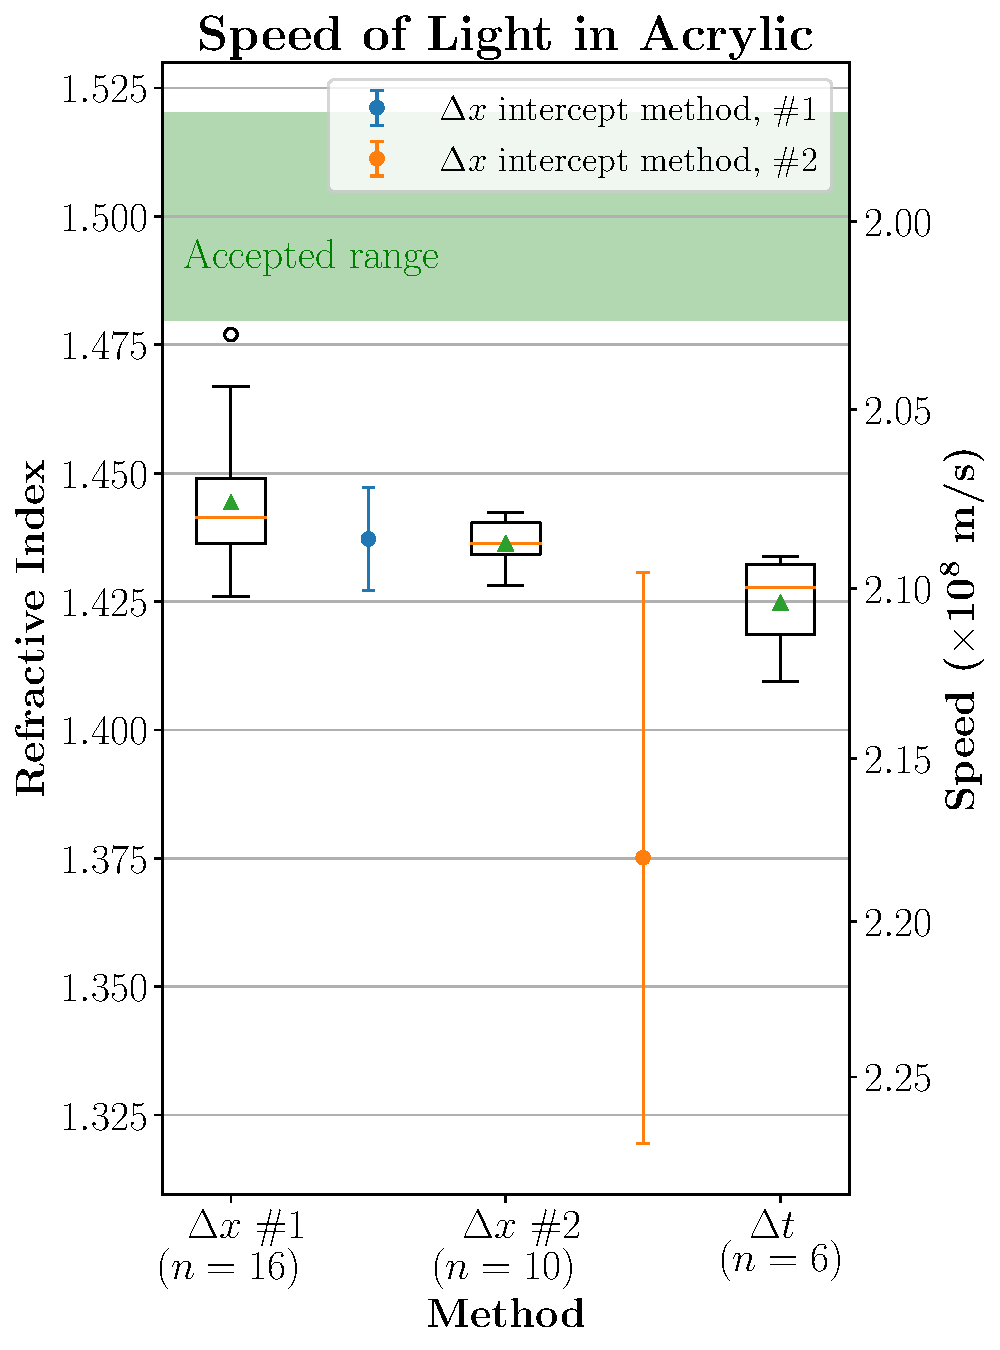
\includegraphics[width=0.7\linewidth]{acrylic}
    \caption{Measured values of the speed of light in PMMA using
        the $\Delta x$ and $\Delta t$ methods. Green triangles are
        the mean values.}
    \label{acrylic_plot}
\end{figure}

None of the measurements are consistent with the literature. Despite
possible variations in manufacturing, the fact that the measurements are
all consistent with each other (the uncertainties shown in Table
\ref{results_table} overlap) indicates again that the measurements
were subject to a systematic error (see Discussion).

The consistency of the results with each other and the similar
magnitudes of their uncertainties support the theoretical
equivalence between the $\Delta x$ and $\Delta t$ methods, but does
not suggest that one is more robust to systematic errors than the other.


\subsection{Water}
The same methods were applied for water as PMMA, with the results shown
in Figure \ref{water_plot}. The result of the intercept method on the
second day is not shown for the same reason.

Four values for $n_\mathrm{H_2O}$ at $\lambda = \SI{630}{\nano\meter}$
from existing literature were considered (data obtained from database
\cite{rii}):
\begin{align*}
    \cite{kedenburg} (\SI{20}{\celsius} \text{, experimental})
    &: 1.3320 \pm 0.0003, \\
    \cite{daimon} (\SI{20}{\celsius} \text{, experimental})
    &: 1.3322, \\
    \cite{hale} (\SI{25}{\celsius} \text{, review})
    &: 1.3318, \text{ and} \\
    \cite{segelstein} (\SI{25}{\celsius} \text{, review/theoretical})
    &: 1.3316;
\end{align*}
these are shown as horizontal lines in Figure \ref{water_plot}.

\begin{figure}[ht]
    \centering
    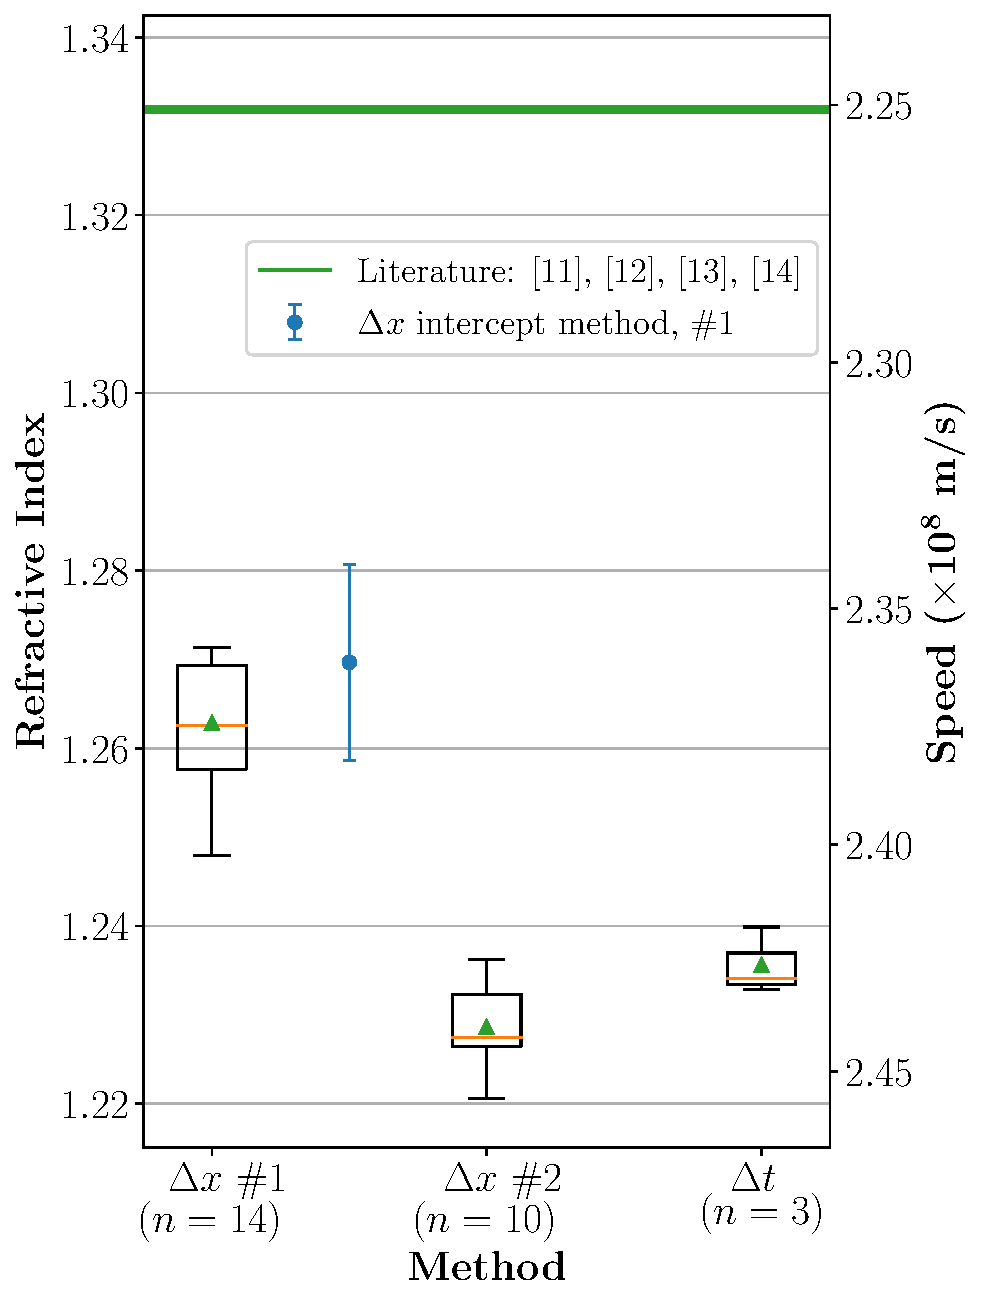
\includegraphics[width=0.7\linewidth]{water}
    \caption{Measured values of the speed of light in water using
        the $\Delta x$ and $\Delta t$ methods. Green triangles are
        the mean values.}
    \label{water_plot}
\end{figure}

As for PMMA, none of the results are consistent with the literature but
the second $\Delta x$ and $\Delta t$ results are still consistent with
each other. Similar conclusions can be drawn regarding the presence of
systematic errors and the equivalence of the $\Delta x$ and $\Delta t$
methods.

~

Table \ref{results_table} summarises all the numerical results of this
report. The $\Delta x$ and $\Delta t$ methods in PMMA and water gave
multiple values; those shown in the table are the averages, with the
uncertainties taken to be the sample standard deviations.
\begin{table}[ht]
    \begin{tabular}{|c|c|c|}
        \hline
        \Centerstack{\textbf{Material} \\ \textbf{(method)}}
        & $n$
        & $c$ ($\times \SI{e8}{\meter \per\second}$) \\
        \hline
        \hline
        Air & $1.019 \pm 0.005$ & $2.941 \pm 0.016$ \\
        \hline
        \hline
        \Centerstack{PMMA \\ ($\Delta x$ \#1)}
        & $1.444 \pm 0.013$ & $2.076 \pm 0.018$ \\
        \hline
        \Centerstack{PMMA \\ ($\Delta x$ intercept \#1)}
        & $1.437 \pm 0.010$ & $2.086 \pm 0.015$ \\
        \hline
        \Centerstack{PMMA \\ ($\Delta x$ \#2)}
        & $1.436 \pm 0.004$ & $2.087 \pm 0.006$ \\
        \hline
        \Centerstack{PMMA \\ ($\Delta t$)}
        & $1.425 \pm 0.009$ & $2.104 \pm 0.014$ \\
        \hline
        \hline
        \Centerstack{Water \\ ($\Delta x$ \#1)}
        & $1.263 \pm 0.007$ & $2.374 \pm 0.013$ \\
        \hline
        \Centerstack{Water \\ ($\Delta x$ intercept \#1)}
        & $1.270 \pm 0.011$ & $2.361 \pm 0.021$ \\
        \hline
        \Centerstack{Water \\ ($\Delta x$ \#2)}
        & $1.229 \pm 0.004$ & $2.440 \pm 0.009$ \\
        \hline
        \Centerstack{Water \\ ($\Delta t$)}
        & $1.236 \pm 0.003$ & $2.426 \pm 0.006$ \\
        \hline
    \end{tabular}
    \caption{Summary of results.}
    \label{results_table}
\end{table}


\section{Discussion}

\subsection{Systematic error sources}

It is notable that the speeds measured in all three media were lower
than the literature values, and by similar amounts (on the order of
$5\%$). This supports the previous conclusions that a systematic error
was present.
Several possibilities are proposed:

\emph{Misalignment.} There was a significant amount of play in the
sliding mechanism of the reflector, making it necessary to support it
with strips of paper to render the reflected beam horizontal. Furthermore,
despite careful efforts to visually align the PMMA and water cylinders
by observing the position of the laser spot at each end, it was very
difficult to ensure that they
were exactly parallel to the beam with the equipment available. Both
factors made it difficult to obtain an accurate measurement of the path
length. A worst-case uncertainty estimate can be derived using Pythagoras'
theorem: if the beam deviates laterally from the axis of the cylinder by
$\SI{2}{\centi\meter}$ at one end and the axis deviates from the ideal
line by $\SI{1}{\centi\meter}$, the increase in path length over
two traversals of the $\SI{50}{\centi\meter}$ cylinder is
\[
    2\left(
        \sqrt{(\SI{3}{\centi\meter})^2 + (\SI{50}{\centi\meter})^2}
        - \SI{50}{\centi\meter}
    \right)
    = \SI{1.8}{\milli\meter}.
\]

\emph{Imperfect cylinder shape.} It is likely that the ends of the
acrylic and water cylinders were not exactly parallel to each other,
causing refraction and increasing the actual path length even with
good alignment. The fact that the observed time difference between
the emitted and reflected beams varied by up to $\SI{40}{\pico\second}$
as the cylinders were rotated supports this hypothesis.
An estimate of the resultant change in apparent refractive index can
be derived from \ref{t_eqn}:
\[
    \delta n = \frac{c \times \SI{40}{\pico\second}}{2l} \approx 0.012.
\]
This is a significant change. The amount of variation was limited by
making a mark on the side of each cylinder so that their orientations
did not change from one measurement to another.

\emph{Phase drift.} During data collection, a systematic drift over time
was observed in the phase difference of the signals from the
source/detector unit, and although the unit was calibrated at the
same reference position before every measurement, the effect was likely
not completely eliminated.

\subsection{Improvements}
The three aforementioned sources of systematic error are all connected
to the fact that the experiment uses a \emph{time of flight} technique;
in one way or another, all the techniques used relied on a measurement
of distance and time. For this reason, a method that relies on the
refraction of light at an interface, such as the deviation and critical
angle methods described in the Introduction, may be more suitable
for PMMA and water.

Consider a simple measurement of the incidence
and refraction angles at an air-material interface; Snell's law
$n_\mathrm{a}\sin{i} = n\sin{r}$ implies an approximate uncertainty,
using the first-order Taylor series method and taking
$i = \ang{45}$, $r = \ang{30}$, $\delta i = \delta r = \ang{0.1}$, of
\begin{align*}
    \delta \left( \frac{n}{n_\mathrm{a}} \right)
    &= \delta \left( \frac{\sin{i}}{\sin{r}} \right) \\
    &= \sqrt{
        \left( \frac{\cos{i}}{\sin{r}} \delta i \right)^2
        + \left( \frac{\sin{i}}{\sin^2{r}} \cos{r} \delta r \right)^2
    } \\
    &\approx 0.005.
\end{align*}
This is similar to the uncertainties presented in this report, but the
method is not subject to unreliable path length or time measurements
and could be inexpensively realised in a teaching laboratory with
a laser source, prism and a target mounted to a goniometer. An
uncertainty of $\ang{0.1}$ in the refraction angle would correspond to
a motion of $\SI{1.7}{\milli\meter}$ at the end of a $\SI{1}{\meter}$
goniometer arm and is hence quite achievable.


\section{Conclusion}

The speed of light and refractive index in air, PMMA and water
were successfully measured, but none were in agreement with literature. The
discrepancy is attributed to a combination of misalignment of the
apparatus, imperfect shape of the PMMA and water cylinders, and
time-dependent drift in readings from the source/detector unit.
The unsatisfactory nature of the result despite careful attempts to
mitigate these errors prompts the proposal of an alternative method
for PMMA and water that measures refraction angles at their interfaces
with air.


\section{Acknowledgements}

The author wishes to thank Prof. Chris Tinney, his fellow
students Marnie Separovich and Winnie Tang, and the five peer referees
of this report for their valuable feedback and suggestions.


\section{Supplements}

The code, raw data and laboratory notebook associated with this report
are available in full at \url{https://github.com/tschanzer/speed_of_light}.


\bibliography{references}

\end{document}
